\documentclass[12pt]{article}
\usepackage[utf8]{inputenc}
\usepackage{amsmath}
\usepackage{graphicx}
\usepackage{listings} % for source code inserts
\title{CS 470 Spring 2011 \\
     Project 3a}
\author{Colby Blair}
\date{Due April 13th, 2011}
\begin{document}
\maketitle

\begin{abstract}
Artificial Neural Networks (ANNs) are one of the most interesting areas of Artificial Intelligence (AI). ANNs 
are useful when other AI solutions become too complex, and are better at tackling more general problems.
ANNs are not as good at solving problems that are specific and don't change as much, compared to other
AI methods. This report uses an ANN to fly a rocket, a problem that has a complex solution.

ANNs are a way to implement learning in AI, and are modeled after the way the human brain functions. Artificial Neurons create a network, and feed inputs into and out of each other. Artificial Neurons then adjust the weights of each of their individual inputs. This learning process eventually matches expected output with
output of the whole network. 

There is one general way of learning, but there are several ways to teach the network. That is, there are 
several ways to tell the network what output you expect for a given input. Some teaching methods are
more intense than others, and some are beyond the scope of this report. In this report, expected values
are generated by a teaching function, developed by the author. The learning algorithm is not perfect, but 
allows implementation of the ANN and understanding of its concepts.
\end{abstract}

\thispagestyle{empty}

\pagebreak

\thispagestyle{empty}
\tableofcontents
\listoffigures

\pagebreak

\setcounter{page}{1}

\section{Introduction}

\subsection{Artificial Neurons (AN)}
An  ANN is a group of nodes, or neurons, that share connections. The neuron itself has several inputs,
of which are weighted. The weights adjust the input, depending on what level of error is believed to exist
on that input. The neuron collects these inputs, runs them through a function, and outputs them to the
next neuron.

\begin{figure}[h]
        \begin{center}
		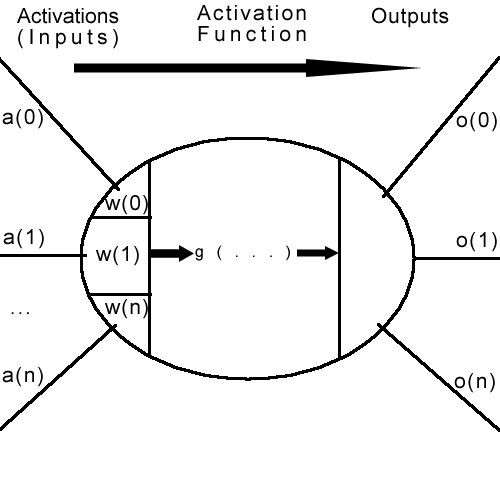
\includegraphics[width=80mm]{report_images/neuron01.png}
                	\caption{An Artificial Neuron}
                	\label{neuron01}
        \end{center}
\end{figure}

\pagebreak

The neuron collects activations (inputs) and weights them. Initially, the weights can be random. Each activation is multiplied by its weight, and all the activation-weight pairs are summed together and fed into 
the activation function $ g() $. In this case, we use the sigmoid function for our activation function.

\begin{figure}[h]
        \begin{center}
		\begin{tabular}{l r}
			$g ( i )$		&	$ = \frac{1}{1 + e^{-i}} $		\\
						&							\\
			where			&						\\
						&	$i  = \sum_{n=1}^1 a_n * w_n$ 	\\

		\end{tabular}
                	\caption{Activation funtion}
                	\label{act_func01}
        \end{center}
\end{figure}

Outputs are all the same value that comes from the activation funtion. They will be different, howerver, coming into the next node, because of how the next node weights them.

Although weights are initially random, they become adjusted so that the node matches an expected output
value. This is gone into detail in Section \ref{sec:learning}.

\subsection{Artificial Neural Networks (ANNs)}
There are several topologies in ANNs. This report implements a \textbf{forward feeding} ANN, although it 
will consider others. A forward feeding network is simpler than other topologies, in that it doesn't have
loopbacks, or inputs that go against the normal flow of output. First, we will consider a forward feeding ANN
with bias (input) nodes, output nodes, and no \textbf{hidden layers}.

\subsection{Feed Forward ANN with no Hidden Layers}

\begin{figure}[h]
        \begin{center}
		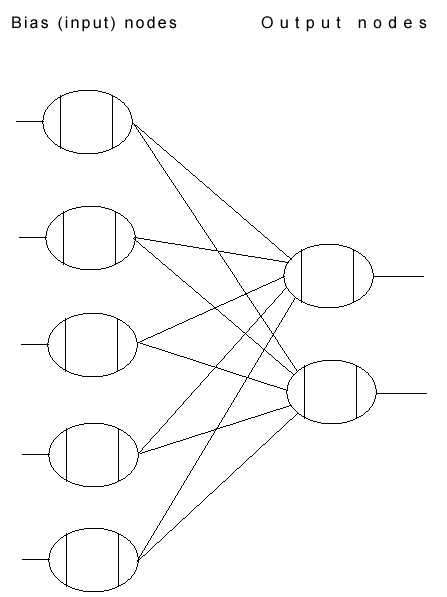
\includegraphics[width=40mm]{report_images/feedforward01.png}
                	\caption{A forward feeding ANN with no hidden layers}
                	\label{feedforward01}
        \end{center}
\end{figure}

Feed forward simply means that no output from a node on the right feeds back into a node on the left. The 
alternative is a \textbf{back propating} ANN. For example, in Figure \ref{feedforward01}, if one of the outputs
from the output nodes then connect into the input of one of the input nodes, back propogation would occur.

In Figure \ref{feedforward01}, there is only biased (input) and output nodes. The biased nodes simply take
the inputs in from a source, i.e. variables for our rocket environment. They apply the $ g() $ activation 
function, and output to the output nodes. The output nodes weight each activation (output from the input
nodes), and apply the $ g() $ activation function. They then output back to the system.

\subsection{Feed Forward ANN with Hidden Layers}

A variation to this ANN is a feed forward ANN with a \textbf{hidden layer}. A hidden layer is just another layer 
between the biased and output nodes. They are not directly inputed from or output to any control system, 
but instead only with other nodes. This creates some trickyness when we try to adjust the weights, as we 
will see in Section \ref{sec:learning}.

\pagebreak

\begin{figure}[h]
        \begin{center}
		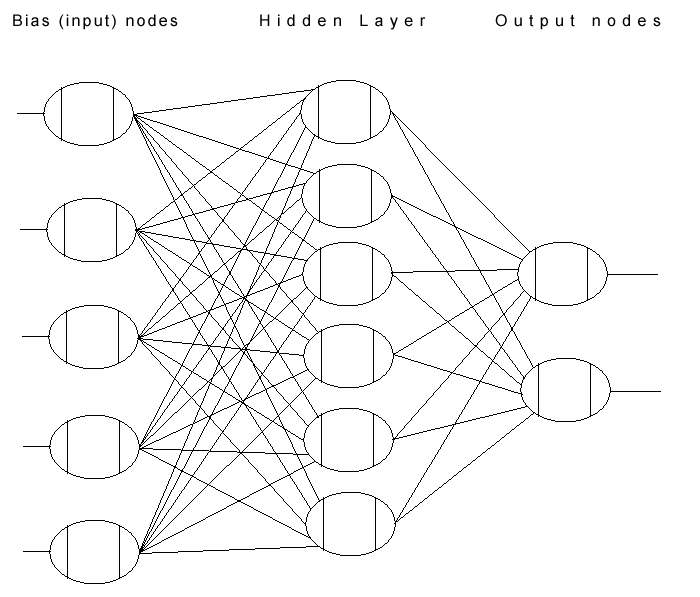
\includegraphics[width=60mm]{report_images/feedforward_hidden01.png}
                	\caption{A forward feeding ANN with one hidden layer}
                	\label{feedforward_hidden01}
        \end{center}
\end{figure}


\section{Learning}
\label{sec:learning}
Learning requires a re-weighting process of each neuron in the ANN. Starting from the right-most (output)
nodes of the ANN, the ANN output is recieved. Our teaching algorithm tells us what value we should
have got. The error is then $ E = Output_{ANN} - Output_{teacher} $. To find the new value for each weight,
we need the equation:

\begin{figure}[h]
        \begin{center}
		\begin{tabular}{r l}
			$w_{n}$		&	$ =  w_{n ( old )} + ( \alpha * a_n * E * \dot g(i) )$	\\
						&										\\
			where		&										\\
						&	$\alpha$ is the learning constant (usually .5)		\\
						&	$a_n$ in the $n^{th}$ activation (input), corresponding with $w_n$ \\
						&	$ E  = $ error  $ = Output_{ANN} - Output_{teacher} $ \\
						&	$ \dot g() $ is the derivative of the activation function $ g() $ \\
						&	... $ g() = \frac{1}{1 + e^{-i}} $				\\
						&	$ \dot g() = \frac{e^{i}}{(1 + e^{i})^2} $			\\
						&	$i  = \sum_{n=1}^1 a_n * w_n$ 	\\
		\end{tabular}
                	\caption{Re-weight function}
                	\label{weight_func}
        \end{center}
\end{figure}

\pagebreak

\begin{figure}[h]
        \begin{center}
		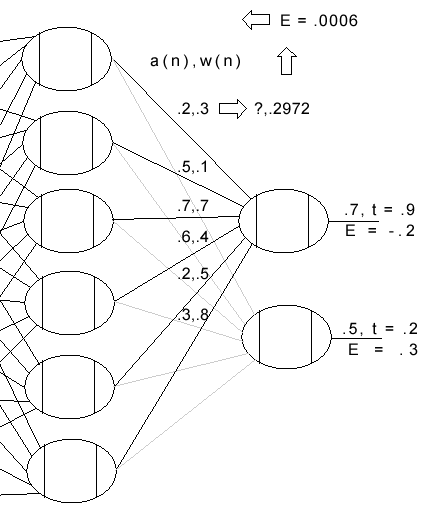
\includegraphics[width=60mm]{report_images/feedforward_hidden02.png}
                	\caption{Re-weighting}
                	\label{feedforward_hidden02}
        \end{center}
\end{figure}

Consider the top output node in Figure \ref{feedforward_hidden02}. Consider one of the weights, $ w_0 $.
To re-weight $w_0$, the calculation would go: \\

	\begin{tabular}{r l}
		$w_{0}$		&	$ =  w_{0 ( old )} + ( \alpha * a_n * E * \dot g(i) )$	\\
					&	$ = .3000 + (.5 * .2 * -.2 * .1798)	$			\\
						% -.003596 %
					&	$ = .2964 $							\\
					&										\\
		where		&										\\
					&	$ \alpha = .5 $ 		\\
					&	$ a_n = .2 $ \\
					&	$ E  = Output_{ANN} - Output_{teacher}  = .7 - .9 = -.2 $ \\
					&	$ \dot g() = \frac{e^{i}}{(1 + e^{i})^2}  = .1798$	\\
						% 3.2544 / (1 + 3.2544) ^ 2 = 3.2544 / 18.1000 = .1798 %
					&	$i  = \sum_{n=1}^1 a_n * w_n = 1.18$			\\
						% .06 + .05 + .49 + .24 + .10 + .24 = 1.18%
	\end{tabular} \\

The values above are arbitrary, but what can be seen is the proportional change of $w_0$ in response to the
error. What should also be noticed is the proportion of change of weight due to the activation (input) that was 
recieved. The higher the error, the higher high activations are penalized. This is analogous with the idea that, 
as a node, "I have a high error, so I must be receiving too much bad information through a high
activation, and not receiving enough good information through a low activation".

If hidden layers do not exist, then the process is done. If they do, then the re-weighted nodes need to 
share their hypothesis about how much error each activation is providing. There are many ways of doing this,
but one way is that our new weight times the current activation would provide our desired $i_{0}$. The 
differece between our desired $i_{0}$ and the real $i_{0}$ is the error we can communicate back to the node:
 
	\begin{tabular}{r l}
		$i_{0,real} $		&	$ = a_{0} * w_{0,old} = .2 * .3	$		\\
						&	$ = .06 $							\\
		$i_{0,desired} $		&	$ = a_{0} * w_{0}	= .2 * .2964$			\\
						&	$ = .0594 $						\\
		$ E $				&	$ = .06 - .0594 = .0006$				\\
	\end{tabular} \\

$w_0$ may not have a lot of error to report up to the next node, because the activation wasn't big. But other
nodes with higher activation will recieve a higher error feedback. The next node will take all reported errors about its output, sum them together, and use that as its error for its own re-weighting.

\subsection{Teaching Algorithm}
\label{sec:teaching}
The teaching algorithm used was fairly simple, and because of this, didn't deliver great results. It would 
deliver both thrust (x movement) and burn (y movement). For thrust, the exponential distance away from
center plus x velocity was used as output. This lightend up on thrust as the rocket centered, and directly 
compensated for any random x velocity caused by wind. For burn, the logarithm of height with base 1/2 plus
the  y velocity was was used. Some tuning was attempted, but never perfected. This attempted to increase
burn when approaching the landing pad, compensating for any random change in y velocity due to random
gravity changes.

\begin{figure}[h]
        \begin{center}
		\begin{tabular}{r l}
			$thrust$		&	$ =  \alpha * e^{{|D_{center}|}} + \phi * v^x $	\\
						&	where $ \alpha =$  -1 left of center, +1 right of center, $\phi$ is a manual adjust \\
			$burn$		&	$ = \beta + log_{1/2}(height) + \omega * v^y $		\\
						&	where  $ \beta,\omega $ are manual adjusts

		\end{tabular}
                	\caption{Teaching Algorithm}
                	\label{teaching_alg}
        \end{center}
\end{figure}

Teaching would be done for the first few iterations in an environment, and then the rocket would be allowed
to try landing. 


\section{Results}
The rocket never reallly did well, as the teaching method never solidified. Even though the success was not
good, the rocket did noticably better with one hidden layer at least. It seems that with more neurons ,there 
were more potential paths to be trained for more variance in inputs. Each hidden layer seemed to add some 
added ability to componsate for randomness in the environment.

It is also notable that even though the teaching algorithm didn't work, the next part of the assignment 
implements a fuzzy logic controller. It would be really great to use the controller as a teacher, and then see
how the ANN does. This is the goal at this point, but would be interesting just to see if it could get the ANN
to work better. Other methods could include using Genetic Algorithms and only evaluating on crashes / 
landings, and other methods of measuring fitness. A fitness function may be just as complex as a teaching
algorithm, however, so it seems like the fuzzy control is a good teaching option for the future of this ANN.

\end{document}
